\documentclass[../../syllabus_2.tex]{subfiles}
\begin{document}

\chapter{Diviseurs et multiples}

\section{Rappels}

Coche la ou les proposition(s) qui corresponde(nt) à la proposition de départ.

\begin{enumerate}
    \item Dans cette division écrite,
          % je ne fais pas la div euclidienne je te laisse haha

          \begin{minipage}{.7\linewidth}
              \begin{enumerate}[cols=2, label={\faIcon[regular]{square}}]
                  \item 423 est le quotient.
                  \item 18 est le diviseur.
                  \item 9 est le dividende.
                  \item 23 est le reste.
              \end{enumerate}
          \end{minipage}
          \hfill
          \begin{minipage}{.2\linewidth}
              $\opidiv[displayintermediary=all,voperation=top]{423}{18}$
          \end{minipage}


    \item Le quotient entier de 100 par 20 est \dots
          \begin{enumerate}[cols=4, label={\faIcon[regular]{square}}]
              \item 80
              \item 120
              \item 2000
              \item 5
          \end{enumerate}

    \item 60 possède \dots
          \begin{enumerate}[cols=4, label={\faIcon[regular]{square}}]
              \item 10 diviseurs
              \item 11 diviseurs
              \item 12 diviseurs
              \item 15 diviseurs
          \end{enumerate}

    \item Si un nombre en divise deux autres, alors \dots
          \begin{enumerate}[cols=2, label={\faIcon[regular]{square}}]
              \item il divise aussi leur somme
              \item il divise aussi leur quotient
              \item il divise aussi leur différence
              \item il divise aussi leur produit
          \end{enumerate}

    \item 16 \dots{} 4
          \begin{enumerate}[cols=2, label={\faIcon[regular]{square}}]
              \item \dots est un multiple de \dots
              \item \dots est un diviseur de \dots
              \item \dots divise \dots
              \item \dots est divisible par \dots
          \end{enumerate}

    \item Un nombre est divisible par 3 si \dots
          \begin{enumerate}[label={\faIcon[regular]{square}}]
              \item il se termine par 3
              \item ses 3 derniers chiffres forment un nombre divisible par 3
              \item la somme de ses chiffres est un nombre divisible par 3
              \item la somme de ses chiffres est un nombre divisible par 9
          \end{enumerate}

    \item Ces deux nombres sont premiers entre eux :
          \begin{enumerate}[cols=4, label={\faIcon[regular]{square}}]
              \item 20 et 15
              \item 13 et 80
              \item 2 et 3
              \item 91 et 28
          \end{enumerate}

    \item 180 =\dots
          \begin{enumerate}[cols=4, label={\faIcon[regular]{square}}]
              \item $2^2\cdot 3\cdot 5^2$
              \item $2^3\cdot 3^2 \cdot 4^2$
              \item $2\cdot 3\cdot 5$
              \item $2^2 \cdot 3^2 \cdot 5$
          \end{enumerate}

    \item Quels sont les nombres premiers  ?
          \begin{enumerate}[cols=4, label={\faIcon[regular]{square}}]
              \item 37
              \item 53
              \item 91
              \item 1
          \end{enumerate}

    \item Je suis un multiple de 4 compris entre 35 et 45.
          \begin{enumerate}[cols=4, label={\faIcon[regular]{square}}]
              \item 40
              \item 36
              \item 42
              \item 44
          \end{enumerate}
\end{enumerate}

\newpage
\section{Division euclidienne}
\begin{exercise}
    C'est Halloween. Joachim a reçu 28 chocolats au caramel, mais il n'aime pas ça. Il décide donc de les partager équitablement entre ses amis~:

    \begin{enumerate}[itemsep=\fill, after=\vfill]
        \item S'il a 5 amis chez lui ce soir-là, combien de chocolats va recevoir chaque ami~? \\
              Combien en restera-t-il dans le sac de Joachim~?
        \item La petite sœur de Joachim arrive au moment du partage. Joachim reprend alors tous ses chocolats et les redistribue en comptant sa petite sœur. Combien chacun des amis et la petite sœur vont-ils recevoir de chocolats~? Va-t-il en rester à Joachim~?
        \item Dans une autre maison, Malik distribue des bonbons à ses 3 amis. Chaque ami en a reçu 6, et il reste 2 bonbons dans la main de Malik. Combien avait-il de bonbons au départ~?
    \end{enumerate}
\end{exercise}
\begin{solution}
    \begin{enumerate}
        \item $\opidiv[displayintermediary=all,voperation=top]{28}{5}$
    \end{enumerate}
\end{solution}

% TODO: pointillé ou un espace blanc pour noter la relation avec les différents noms ?
Il existe une égalité qui permet de retrouver le dividende à partir du diviseur, du reste et du quotient. Quelle est-elle ?

\dotsforanswer{1}

\newpage
\begin{exercise}
    Lylia, Dina, Camille et Esther aimeraient jouer à bataille. Pour que le jeu soit équitable, chaque joueur doit posséder le même nombre de cartes au départ.
    \begin{center}
        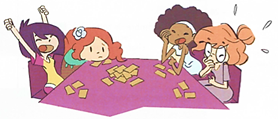
\includegraphics{img/cartes.png}
    \end{center}
    \begin{enumerate}[itemsep=\fill, after=\vfill]
        \item \textbf{Première partie :} si elles doivent se partager équitablement les 52 cartes que contient un jeu, combien de cartes recevront-elles chacune ? Combien de cartes ne seront pas distribuées ?
        \item \textbf{Deuxième partie :} Marie vient se joindre à elles. Combien de cartes recevront-elles alors chacune ? Combien de cartes ne seront pas distribuées ?
        \item \textbf{Troisième partie :} les filles sont toujours à cinq à jouer et Lylia distribue les 52 cartes, mais il lui en reste 7 dans les mains. Les a-t-elle distribuées correctement ? Explique.
    \end{enumerate}
\end{exercise}

Il existe donc une condition concernant le reste d'une division euclidienne. Quelle est-elle~?

\dotsforanswer{2}

\newpage
La division euclidienne est une division écrite qui répond à une égalité
et une condition~:
\vspace{7cm}

%ajouter de l'espace pour une division euclidienne à la main
Égalité~:

Condition~:

Qu'est-ce qu'une division exacte ?
\dotsforanswer{2}

\begin{exercise}
    Effectue les divisions euclidiennes suivantes, et écris l'égalité qui en découle.
    \begin{enumerate}[cols=3]
        \item $59 : 3$
        \item $829 : 4$
        \item $834 : 7$
    \end{enumerate}
\end{exercise}

\newpage

\begin{exercise}
    Quel est le nom de 19 dans les égalités euclidiennes suivantes?\\
    \begin{enumerate}[itemsep=1em]
        \item $139=20\cdot 6+19$\hfill\dotfillbox[8cm]
        \item $19=3\cdot 5+4$\hfill\dotfillbox[8cm]
        \item $499=25\cdot 19+24$\hfill\dotfillbox[8cm]
        \item $81=4\cdot 19+5$\hfill\dotfillbox[8cm]
    \end{enumerate}
\end{exercise}

\begin{exercise}
    Complète le tableau ci-dessous.
    \begin{center}
        $\begin{tblr}{
                    hlines,
                    vlines,
                    rows={1cm,m},
                    row{1}={gray!40, font=\bfseries},
                    columns={c ,1cm},
                    column{5}={7cm}
                }
                \text{D} & \text{d} & \text{q} & \text{r} & \text{Égalité} \\
                56       & 9        &          &          &                \\
                         & 8        & 4        & 3        &                \\
                57       &          & 14       &          &                \\
                85       &          &          & 8        &                \\
                         &          &          &          & 39=5\cdot 7+4  \\
                         &          &          &          & 26=3\cdot 7+5  \\
            \end{tblr}$
    \end{center}
\end{exercise}


\begin{exercise}
    Dans une division euclidienne, le diviseur est 7, le quotient est 5 et le reste vaut 3. Quel est le dividende? \\
    \vspace{4cm}
\end{exercise}
\newpage
\begin{exercise}
    L'ensemble des élèves de deuxième année et 5 professeurs aimeraient partir en excursion dans un parc d'attractions.
    \begin{enumerate}[itemsep=3cm]
        \item Sachant qu'il y a 225 élèves en deuxième année, et qu'un car ne peut transporter que 35 personnes, combien de cars faudra-t-il réserver? Écris tous tes calculs.
        \item Combien de places resteront inoccupées?
        \item Voici un tableau reprenant les tarifs dans le parc d'attraction. Combien faudra-t-il débourser à la caisse? Écris tous tes calculs.
              \begin{center}
                  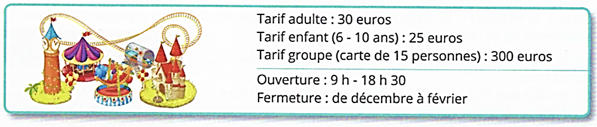
\includegraphics{img/prix.png}
              \end{center}
    \end{enumerate}
\end{exercise}
\newpage
\begin{exercise}
    Transforme ces minutes en heures et minutes. Utilise la division euclidienne.
    \begin{enumerate}[cols=3]
        \item $\SI{179}{min}$
        \item $\SI{813}{min}$
        \item $\SI{1670}{min}$
    \end{enumerate}
    \vspace{5cm}
\end{exercise}

\begin{exercise}
    Vingt-sept pirates décident de se partager leur dernier butin composé de 386 pièces d'or. John le Borgne, le plus âgé et le plus malin de tous, dit à ses compagnons~:
    \begin{emph}
        \og~Partagez ces pièces d'or entre vous de manière équitable et je prendrai ce qu'il restera~\fg
    \end{emph}
    Détermine la part de chaque pirate ainsi que celle de John le Borgne. Écris tous tes calculs.
    \vspace{5 cm}
\end{exercise}

\begin{exercise}
    Encadre ces fractions par deux entiers consécutifs.
    \begin{enumerate}[cols=2]
        \item $ \dots < \dfrac{23}{7} < \dots $
        \item $ \dots < \dfrac{66}{9} < \dots $
        \item $ \dots < \dfrac{47}{87} < \dots $
        \item $ \dots < \dfrac{-51}{6} < \dots $
    \end{enumerate}
\end{exercise}

\newpage

\section{Expressions littérales}
Pour chacun des énoncés ci-dessous, écris l'expression générale qui le traduit en utilisant $n$ pour désigner n'importe quel nombre entier.
\begin{enumerate}[itemsep=1em]
    \item 3 nombres consécutifs :\dotfill
    \item Un nombre pair :\dotfill
    \item Un nombre impair :\dotfill
    \item Deux nombres pairs consécutifs :\dotfill
    \item Trois nombres impairs consécutifs :\dotfill
    \item Un multiple de 3 :\dotfill
    \item Deux multiples de 5 consécutifs :\dotfill
    \item Un multiple de 9 augmenté de 1 :\dotfill
\end{enumerate}

\begin{exercise}
    Pour les expressions suivantes, Coche la ou les cases adéquates.
    \begin{center}
        \begin{tblr}{
                hlines,
                vlines,
                row{1}={gray!40},
            }
            Expression & $ 3\mathbb{N}$ & $4\mathbb{N}$ & $5\mathbb{N}$ \\
            $5n$       &                &                               \\
            $4n+4$     &                &                               \\
            $6n+12$    &                &                               \\
            $3n+27$    &                &                               \\
            $40n$      &                &                               \\
            $15n$      &                &                               \\
            $24n$      &                &                               \\
            $20n+20$   &                &
        \end{tblr}
    \end{center}
\end{exercise}

\begin{exercise}
    Vrai ou faux? Justifie dans tous les cas.
    \begin{enumerate}
        \item Le nombre 0 est un nombre pair.
              \dotsforanswer{2}
        \item $n + 5$ est un nombre naturel dont le chiffre des unités est $5$.
              \dotsforanswer{2}
        \item $21n + 11$ est un multiple de $7$.
              \dotsforanswer{2}
        \item $12n$ est multiple de 4.
              \dotsforanswer{2}
        \item $12n + 18$ est un multiple de $6$.
              \dotsforanswer{2}
    \end{enumerate}
\end{exercise}
\newpage
\section{Propriétés mathématiques}

Grâce aux expressions littérales, nous pouvons prouver des propriétés mathématiques. Pour cela, nous devons utiliser les expressions littérales générales (vraies pour n'importe quel naturel choisi).

\exemple
Prouve que la somme de 4 naturels consécutifs est un nombre pair.
\begin{center}
    \begin{tblr}{
            hlines,
            vlines,
            columns={.45\linewidth,l},
            rows={1cm,m},
            row{1}={gray!40, font=\bfseries}
        }
        Étapes                                                                           & Exemples \\
        Noter l'expression littérale qui correspond aux éléments traités                 &          \\
        Y appliquer l'opération demandée                                                 &          \\
        Développer et réduire le résultat de sorte d'arriver à la conclusion de l'énoncé &          \\
    \end{tblr}
\end{center}

\begin{exercise}
    Prouve les affirmations suivantes à l'aide des expressions littérales.
    \begin{enumerate}[itemsep=\fill, after=\vfill]
        \item La somme de deux nombres naturels impairs est un nombre pair.
        \item La somme de 5 nombres naturels pairs consécutifs est un multiple de 10.
    \end{enumerate}
\end{exercise}

\newpage

\begin{exercise}
    Résous les problèmes ci-dessous. Écris tous tes calculs.
    \begin{enumerate}[itemsep=\fill, after=\vfill]
        \item La somme de deux nombres consécutifs vaut 95. Quels sont ces nombres?
        \item La somme de quatre multiples de 7 consécutifs vaut 406. Quels sont ces nombres?
    \end{enumerate}
\end{exercise}

\newpage

\section{Plus grand commun diviseur (PGCD)}

Mariette désire ranger ses constructions en Lego dans un coffre dont les dimensions sont de \SI{24}{cm} x \SI{36}{cm} x \SI{60}{cm}. Elle veut y introduire des boites cubiques de taille identique, et en remplissant tout l'espace.
\begin{center}
    \includegraphics[width=.5\linewidth]{figures/coffre.tikz}
\end{center}

\begin{enumerate}
    \item Quelles peuvent être les dimensions de ces cubes (si on ne prend que les dimensions entières de centimètres) ?\vspace*{2cm}
    \item Quelles sont les plus grandes dimensions possibles ?
    \item Combien y aura-t-il de cubes de cette dimension dans le coffre ?\vspace*{4cm}
\end{enumerate}
Il existe un moyen de trouver directement la réponse à la question $b$ à l'aide de la décomposition en facteurs premiers de 24, 36 et 60 :

\newpage
Qu'est-ce que le PGCD de deux nombres ou plus?
\dotsforanswer{2}

Notation : \dotfill\medbreak

Il existe trois méthodes pour trouver le PGCD de deux ou de plusieurs nombres.
\begin{itemize}[label=$\bullet$, itemsep=5cm]
    \item Comparaison de tous les diviseurs communs.\\
          \exemple Trouve le PGCD de 16 et 20.

    \item Décomposition de chaque nombre en produits de facteurs premiers. \\
          \exemple Trouve le PGCD de 144 et 360.

    \item Décomposition \og commune\fg{} en facteurs premiers.\\
          \exemple Trouve le PGCD de 105, 45 et 315.
\end{itemize}

\newpage
\section{Propriétés du PGCD}

Déduis des propriétés en observant les nombres de départ et leur PGCD.

\begin{enumerate}[cols=2]
    \item PGCD de 8 et de 40
    \item PGCD de 3 et de 39
\end{enumerate}
\vfill
\dotsforanswer{3}[Propriété 1 : ]

\begin{enumerate}[cols=2]
    \item PGCD de 8 et de 15
    \item PGCD de 2 et de 21
\end{enumerate}
\vfill
\dotsforanswer{3}[Propriété 2 : ]

\newpage

\begin{exercise}
    Détermine les PGCD des nombres suivants. Écris tous tes calculs.
    \begin{enumerate}[cols=2, itemsep= 5cm]
        \item 45 et 7
        \item 120 et 144
        \item 540 et 168
        \item 80 et 320
        \item 60, 48 et 160
        \item 225, 75 et 525
    \end{enumerate}
    \vspace{5cm}
\end{exercise}

\begin{exercise}

    À quelle condition un nombre est-il divisble par les nombres suivants ?
    \begin{enumerate}
        \item 18 ? \dotfill
        \item 40 ? \dotfill
        \item 36 ? \dotfill
    \end{enumerate}
\end{exercise}

\begin{exercise}
    Jusitifie que 285 est divisible par 15 à l'aide des nombres premiers entre eux.
    \dotsforanswer{3}
\end{exercise}

\begin{exercise}
    Quelle est la valeur du symbole $\diamond$  pour que le nombre $328\diamond$  soit divisible par 12? Justifie.
    \adf{8}
\end{exercise}

\begin{exercise}
    Quelle est la phrase correcte? Pour celle qui est incorrecte, donne un contre-exemple.
    \begin{enumerate}
        \item Si deux nombres sont premiers entre eux, alors ils sont également premiers.
        \item Si deux nombres sont premiers, alors ils sont également premiers entre eux.
    \end{enumerate}
    \adf[Contre-exemple :]{1}
\end{exercise}

\newpage
\section{Plus petit commun multiple (PPCM)}
Charles désire ranger des boîtes d'allumettes dans une caisse en carton de forme cubique sans gaspiller l'espace de cette caisse. Les dimensions de ces boîtes d'allumettes sont \SI{4}{cm}~x~\SI{8}{cm}~x~\SI{10}{cm} (comme illustré ci-dessous).
\begin{center}
    \includegraphics[width=.5\linewidth]{figures/allumette.tikz}
\end{center}

\begin{enumerate}
    \item Quelles pourraient être les dimensions (en nombre entier de centimètres) de la caisse en carton? \vspace*{2cm}

    \item Quelles sont les plus petites dimensions possibles ?

    \item Combien de boites d'allumettes peut-on mettre?\vspace*{4cm}
\end{enumerate}
Il existe un moyen de trouver la réponse à la question $b$, directement avec la décomposition en facteurs premiers de 4, 8 et 10 :

\newpage
Qu'est-ce que le PPCM de deux nombres ou plus?
\dotsforanswer{2}
Notation : \dotfill

Il existe trois méthodes pour trouver le PPCM de deux ou de plusieurs nombres.
% Pour chaque méthode, laisser bien de la place pour faire un exemple complet de la méthode avec les nombres en exemple.
\begin{itemize}[label=$\bullet$, itemsep=\fill, after=\vfill]
    \item Comparaison des ensembles des multiples.\\
          \exemple Trouve le PPCM de 16 et 20.

    \item Décomposition de chaque nombre en produits de facteurs premiers. \\
          \exemple Trouve le PPCM de 36 et 60.

    \item Décomposition "commune" en facteurs premiers.\\
          \exemple Trouve le PPCM de 24,36 et 60.
\end{itemize}
\newpage

\section{Propriétés du PPCM}

Déduis des propriétés en observant les nombres de départ et leur PPCM

\begin{enumerate}[cols=2]
    \item PPCM de 8 et de 40
    \item PPCM de 3 et de 39
\end{enumerate}
\vfill
\dotsforanswer{3}[Propriété 1 : ]

\begin{enumerate}[cols=2]
    \item PPCM de 8 et de 15
    \item PPCM de 2 et de 21
\end{enumerate}
\vfill
\dotsforanswer{3}[Propriété 2 : ]

\newpage

\begin{exercise}
    Détermine les PPCM des nombres suivants. Écris tous tes calculs.
    %Mettre bcp d'espace
    \begin{enumerate}[cols=2, itemsep=.3\textheight]
        \item 81 et 19
        \item 27 et 12
        \item 250 et 50
        \item 68 et 72
        \item 12, 36 et 30
        \item 15, 75 et 45
    \end{enumerate}
\end{exercise}

\newpage
\section{Exercices mélangés}
\setcounter{exercise}{0}
\subsection{Exercices de drill}
\activatecollection{div-mul-exos}
\begin{exercise}
    Décompose les nombres suivants en un produit de facteurs premiers.
    \begin{enumerate}[cols=3]
        \item $180$
        \item $360$
        \item $54$
        \item $77$
        \item $120$
        \item $48$
        \item $128$
        \item $\num{2048}$
        \item $91$
        \item $144$
        \item $630$
        \item $64$
    \end{enumerate}
\end{exercise}
\begin{solution}
    \begin{enumerate}[cols=3]
        \item $180 = 2^2 \cdot 3^2 \cdot 5$
        \item $360 = 2^3 \cdot 3^2 \cdot 5$
        \item $54 = 2 \cdot 3^3$
        \item $77 = 7 \cdot 11$
        \item $120 = 2^3 \cdot 3 \cdot 5$
        \item $48 = 2^4 \cdot 3$
        \item $128 = 2^7$
        \item $\num{2048} = 2^11$
        \item $91 = 7 \cdot 13$
        \item $144 = 2^4 \cdot 3^2$
        \item $630 = 2 \cdot 3^2 \cdot 5 \cdot 7$
        \item $64 = 2^6$
    \end{enumerate}
\end{solution}

\begin{exercise}
    Effectue les divisions euclidiennes suivantes et écris l'égalité euclidienne qui en découlent.
    \begin{enumerate}[cols=3]
        \item $\num{186} : 5$
        \item $\num{8652} : 11$
        \item $\num{657} : 3$
        \item $\num{8756} : 20$
        \item $\num{86} : 6$
        \item $\num{946} : 12$
        \item $\num{308} : 6$
        \item $\num{1685} : 5$
        \item $\num{242424} :12$
        \item $\num{9063} : 7 $
        \item $\num{658} : 12$
        \item $\num{1385} : 15$
    \end{enumerate}
\end{exercise}
\begin{solution}
    \begin{enumerate}[cols=3]
        \item $\opidiv[displayintermediary=all,voperation=top]{186}{5}$\medbreak $186=5\cdot37+1$
        \item $\opidiv[displayintermediary=all,voperation=top]{8652}{11}$\medbreak $8652=11\cdot786+6$
        \item $\opidiv[displayintermediary=all,voperation=top]{657}{3}$\medbreak $657=3\cdot219+0$
        \item $\opidiv[displayintermediary=all,voperation=top]{8756}{20}$\medbreak $8756=20\cdot437+16$
        \item $\opidiv[displayintermediary=all,voperation=top]{86}{6}$\medbreak $86=6\cdot14+2$
        \item $\opidiv[displayintermediary=all,voperation=top]{946}{12}$\medbreak $946=12\cdot78+10$
        \item $\opidiv[displayintermediary=all,voperation=top]{308}{6}$\medbreak $308=6\cdot51+2$
        \item $\opidiv[displayintermediary=all,voperation=top]{1685}{5}$\medbreak $1685=5\cdot337+0$
        \item $\opidiv[displayintermediary=all,voperation=top]{242424}{12}$\medbreak $242424=12\cdot20202+0$
        \item $\opidiv[displayintermediary=all,voperation=top]{9063}{7}$\medbreak $9063=7\cdot1294+5$
        \item $\opidiv[displayintermediary=all,voperation=top]{658}{12}$\medbreak $658=12\cdot54+10$
        \item $\opidiv[displayintermediary=all,voperation=top]{1385}{15}$\medbreak $1385=15\cdot92+5$
    \end{enumerate}
\end{solution}

\begin{exercise}
    Écris l'expression générale des expressions suivantes.
    \begin{enumerate}[cols=3]
        \item Un nombre pair.
        \item Trois multiples de 7 consécutifs.
        \item La somme de deux nombres impairs consécutifs.
        \item Un multiple de 6 augmenté de 1.
        \item Un multiple de 5.
        \item Un nombre impair.
        \item Deux multiples de 3 différents.
        \item Un multiple de 10 augmenté de 3.
        \item La différence entre deux nombres pairs consécutifs.
        \item Deux multiples de 5 consécutifs.
        \item Deux nombres impairs différents et non consécutifs.
        \item La somme d'un multiple de 11 et d'un multiple de 4.
        \item Deux nombres pairs consécutifs.
    \end{enumerate}
\end{exercise}
\begin{solution}
    \begin{enumerate}[cols=3]
        \item $2n$
        \item $7n$,$7n+7$ et $7n+14$
        \item $(2n+1) + (2n+3) = 4n+4$
        \item $6n+1$
        \item $5n$
        \item $2n+1$
        \item $3n$ et $3n+3$
        \item $10n+3$
        \item $2n+2 - (2n) = 2$
        \item $5n$ et $5n+5$
        \item $2n+1$ et $2n+5$
        \item $11n + 4n$ %FIXME: problématique dans l'écriture car on a tendance à croire que ça donne un multiple de 15 or c'est faux.
        \item $2n$ et $2n+2$
    \end{enumerate}
\end{solution}

\pagebreak
\begin{exercise}
    Calcule les PGCD des nombres suivants.
    \begin{enumerate}[cols=3]
        \item $84$ et $12$
        \item $75, 125$ et $300$
        \item $14$ et $15$
        \item $900$ et $360$
        \item $9,30$ et $15$
        \item $100$ et $50$
        \item $625$ et $650$
        \item $81$ et $540$
        \item $18, 36$ et $66$
        \item $144$ et $288$
        \item $17$ et $23$
        \item $180$ et $168$
    \end{enumerate}
\end{exercise}
\begin{solution}
    \begin{enumerate}[cols=4]
        \item  $12$
        \item $25$
        \item $1$
        \item $180$
        \item $3$
        \item $50$
        \item $25$
        \item $27$
        \item $6$
        \item $144$
        \item $1$
        \item $12$
    \end{enumerate}

\end{solution}

\begin{exercise}
    Calcule les PPCM des nombres suivants.
    \begin{enumerate}[cols=3]
        \item $40$ et $16$
        \item $75$ et $90$
        \item $90$ et $48$
        \item $80$ et $84$
        \item $44$ et $55$
        \item $150$ et $300$
        \item $2$ et $3$
        \item $12$ et $15$
        \item $50$ et $75$
        \item $16$ et $12$
        \item $14$ et $10$
        \item $60$ et $35$
    \end{enumerate}
\end{exercise}
\begin{solution}
    \begin{enumerate}[cols=4]
        \item $80$
        \item $450$
        \item $720$
        \item $1680$
        \item $220$
        \item $300$
        \item $6$
        \item $60$
        \item $150$
        \item $48$
        \item $70$
        \item $420$
    \end{enumerate}
\end{solution}

\newpage
\subsection{À toi de jouer}
\begin{exercise}
    Quelle(s) est/sont les relations qui représentent une division euclidienne ?
    \begin{enumerate}
        \item $D = r\cdot d + q$\qquad avec $r<d$
        \item $D = d\cdot q + r$\qquad avec $D<r$
        \item $D = d\cdot q + r$\qquad avec $r>d$
        \item $D = d\cdot q + r$\qquad avec $r<d$
    \end{enumerate}
\end{exercise}
\begin{exercise}
    Les égalités suivantes décrivent des divisions euclidiennes. Quel nom porte le nombre 19 dans ces divisions.
    \begin{enumerate}[cols=2]
        \item $139 = 20\cdot 6 + 19$
        \item $19 = 3\cdot 5 + 4$
        \item $499 = 25\cdot 19 + 24$
        \item $81 = 4\cdot 19 + 5$
    \end{enumerate}
\end{exercise}

\begin{exercise}
    Détermine la valeur des lettres dans le tableau suivant.
    \begin{center}
        \begin{tblr}{hlines, vlines, cells={c}, row{1}={font=\bfseries}}
            Dividende & Diviseur & Quotient & Reste \\
            82        & 5        & A        & B     \\
            C         & 10       & 7        & 4     \\
            D         & 8        & 12       & 0     \\
            E         & 8        & 0        & 4     \\
            45        & F        & 11       & 1     \\
        \end{tblr}
    \end{center}
\end{exercise}

\begin{exercise}
    Écris la relation euclidienne pour les divisions suivantes.
    \begin{enumerate}[cols=4]
        \item $1728:4$
        \item $874:3$
        \item $723:12$
        \item $5379:13$
    \end{enumerate}
\end{exercise}

\begin{exercise}
    Détermine le PGCD et le PPCM des nombres suivants.
    \begin{enumerate}[cols=4]
        \item 12 et 26
        \item 48 et 120
        \item 52 et 104
        \item 81 et 17
        \item 28 et 27
        \item 3 et 7
        \item 120 et 150
        \item 10 et 11
        \item 66 et 24
        \item 25, 35 et 45
        \item 144, 72 et 48
        \item 14, 11 et 22
    \end{enumerate}
\end{exercise}

\begin{exercise}
    Combien de tentes de 6 places faut-il pour que les 75 scouts du camp d'unité puissent loger~? Combien restera-t-il de places libres~?
\end{exercise}

\begin{exercise}
    Guillaume souhaite mettre des bonbons dans des sachets pour les offrir à ses copains de classe. Il possède $96$ cerises citriques, $216$ grenouilles et $72$ Dragibus. Il désire confectionner le plus grand nombre de sachets contenant tous le même nombre de bonbons de chaque sorte.
    \begin{tasks}
        \task Détermine le nombre de sachets qu'il peut réaliser pour qu'il ne reste aucun bonbon.
        \task Détermine le nombre de bonbons de chaque sorte contenu dans un sachet.
    \end{tasks}
\end{exercise}

\begin{exercise}
    Valentin possède trois planches de \SI{10}{cm} de large. La première mesure \SI{1,80}{m}, la deuxième \SI{2,40}{m} et la troisième \SI{1,68}{m}. Il voudrait les scier toutes les trois en morceaux de même longueur~; cette longueur doit être la plus grande possible, un nombre entier de centimètres. Quel est le plus grand morceau possible~?
\end{exercise}

\begin{exercise}
    Un numéro de carte d'identité est composé de $12$ chiffres répartis en trois parties. Les deux derniers chiffres représentent toujours le reste de la division par $97$ du nombre formé par les dix premiers chiffres. Vérifie l'exactitude des numéros des cartes d'identité ci-dessous.
    \begin{tasks}
        \task 247-1028457-17
        \task 138-4376001-52
    \end{tasks}
\end{exercise}

\begin{exercise}
    Deux voitures partent en même temps de la ligne de départ et font plusieurs tours du même circuit. La voiture jaune réalise un tour de circuit en 36 minutes tandis que la voiture verte réalise un tour de circuit en 48 minutes. À quel moment les deux voitures vont-elles repasser la ligne de départ ensemble~?
\end{exercise}

\begin{exercise}
    Quel est le plus petit carré que l'on peut former avec des rectangles de \SI{12}{cm} x \SI{16}{cm}~? \\ Combien de rectangles seront utilisés~?
\end{exercise}

\begin{exercise}
    Dans la salle de bain de Juliette, deux robinets coulent goutte à goutte. Le robinet d'eau chaude laisse tomber une goutte toutes les 18 secondes tandis que le robinet d'eau froide en laisse tomber une toutes les 15 secondes.\\
    Juliette remarque qu'à 13h50, les deux robinets ont laissé tomber une goutte en même temps. À quelle heure cela se reproduira-t-il~?
\end{exercise}

\begin{exercise}
    À l'occasion de la fancy-fair, le cuisinier de l'école confectionne de grandes pizzas rectangulaires. Pour leur cuisson, il utilise une plaque rectangulaire de \SI{108}{cm} sur \SI{84}{cm}. Détermine le nombre minimum de parts carrées identiques qu'il peut obtenir en découpant une de ces grandes pizzas et en évitant les déchets. Les dimensions de ces mini pizzas doivent être exprimées en nombre entier de centimètres. \\
    Écris tous tes calculs.
\end{exercise}

\begin{exercise}
    Un entrepreneur doit couvrir le sol d'une salle de bain rectangulaire de \SI{5,94}{m} sur \SI{3,63}{m} avec des dalles carrées dont les côtés se mesurent avec un nombre entier de centimètres.
    \begin{tasks}
        \task Quelle est la taille maximale de dalles carrées qui couvrent exactement la surface de cette salle de bain~?
        \task Combien de dalles de cette taille doit-il utiliser~?
    \end{tasks}
\end{exercise}

\begin{exercise}
    Une briqueterie livre des briques de \SI{16}{cm} x \SI{8}{cm} x \SI{5}{cm} dans des boîtes cubiques (cela facilite le stockage et le transport).
    \begin{tasks}
        \task Quelles sont les dimensions de la plus petite caisse cubique qui conviendra~?
        \task Combien de briques contiendra-t-elle~?
    \end{tasks}
\end{exercise}

\begin{exercise}
    Prouve les affirmations suivantes~:
    \begin{tasks}
        \task La somme de trois nombres consécutifs est multiple de $3$.
        \task La somme de deux multiples consécutifs de $5$ est un multiple de $5$.
    \end{tasks}
\end{exercise}
\deactivatecollection{div-mul-exos}
\newpage
% \printsolutions[collection=div-mul-exos]
\end{document}